\hypertarget{ClientTcpComBny_8cpp}{}\section{Référence du fichier src/\+Client\+Tcp\+Com\+Bny.cpp}
\label{ClientTcpComBny_8cpp}\index{src/\+Client\+Tcp\+Com\+Bny.\+cpp@{src/\+Client\+Tcp\+Com\+Bny.\+cpp}}
{\ttfamily \#include $<$cstdarg$>$}\newline
{\ttfamily \#include $<$unistd.\+h$>$}\newline
{\ttfamily \#include $<$string.\+h$>$}\newline
{\ttfamily \#include $<$sys/types.\+h$>$}\newline
{\ttfamily \#include $<$sys/socket.\+h$>$}\newline
{\ttfamily \#include $<$netinet/in.\+h$>$}\newline
{\ttfamily \#include $<$arpa/inet.\+h$>$}\newline
{\ttfamily \#include $<$Client\+Tcp\+Com\+Bny.\+h$>$}\newline
{\ttfamily \#include $<$Tcp\+Com\+Bny.\+h$>$}\newline
Graphe des dépendances par inclusion de Client\+Tcp\+Com\+Bny.\+cpp\+:
\nopagebreak
\begin{figure}[H]
\begin{center}
\leavevmode
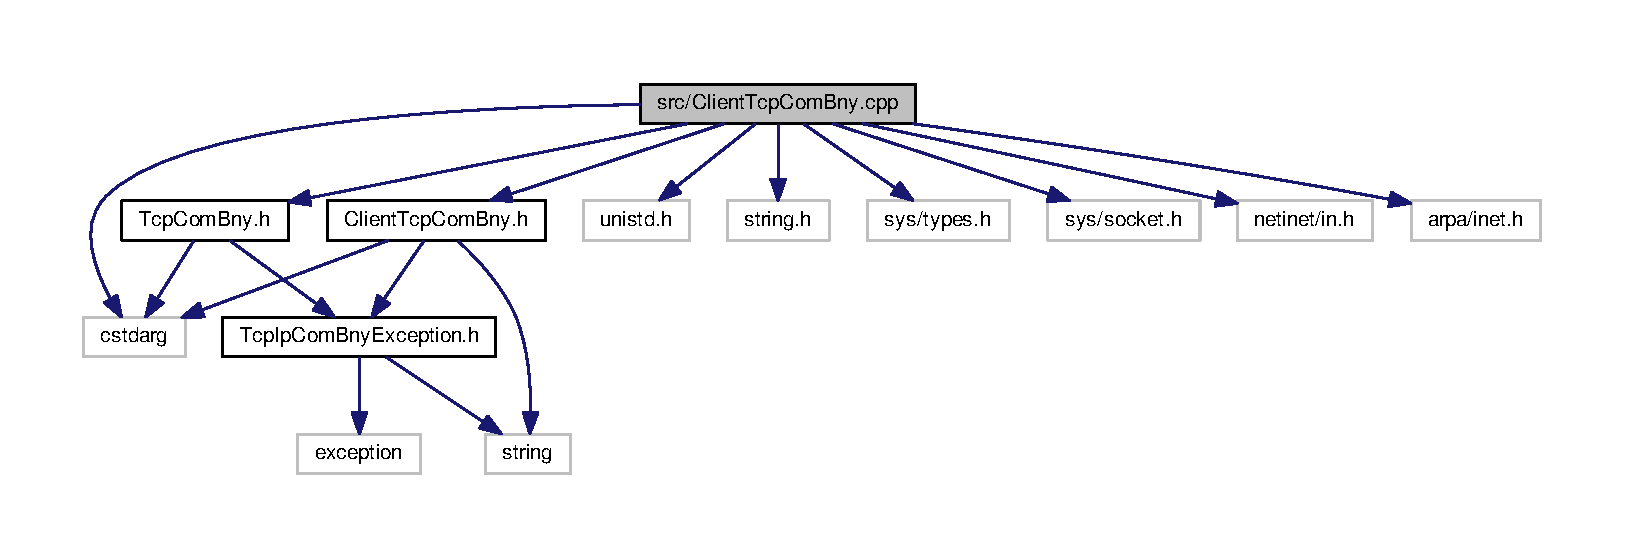
\includegraphics[width=350pt]{ClientTcpComBny_8cpp__incl}
\end{center}
\end{figure}
